\documentclass[12pt, twoside]{article}
\usepackage[letterpaper, margin=1in, headsep=0.2in]{geometry}
\setlength{\headheight}{0.6in}
%\usepackage[english]{babel}
\usepackage[utf8]{inputenc}
\usepackage{microtype}
\usepackage{amsmath}
\usepackage{amssymb}
%\usepackage{amsfonts}
\usepackage{siunitx} %units in math. eg 20\milli\meter
\usepackage{yhmath} % for arcs, overparenth command
\usepackage{tikz} %graphics
\usetikzlibrary{quotes, angles}
\usepackage{graphicx} %consider setting \graphicspath{{images/}}
\usepackage{parskip} %no paragraph indent
\usepackage{enumitem}
\usepackage{multicol}
\usepackage{venndiagram}

\usepackage{fancyhdr}
\pagestyle{fancy}
\fancyhf{}
\renewcommand{\headrulewidth}{0pt} % disable the underline of the header
\raggedbottom
\hfuzz=2mm %suppresses overfull box warnings

\usepackage{hyperref}

\fancyhead[LE]{\thepage}
\fancyhead[RO]{\thepage \\ Name: \hspace{4cm} \,\\}
\fancyhead[LO]{BECA / Dr. Huson / Geometry\\*  Unit 11: Circle angles, sectors, arcs \\* 3 March 2023}

\begin{document}

\subsubsection*{11.5 Homework: Inscribed angle theorem}
\begin{enumerate}
  \item A square is inscribed in a circle with a radius $r=6$. Find each:
  \begin{multicols}{2}
  \raggedcolumns
  \begin{enumerate}[itemsep=1.1cm]
    \item $m \angle AOB$
    \item The circle circumference. ($C=2\pi r$)
    \item The length of the arc $\wideparen{AB}$
    \item The circle's area. ($A=\pi r^2$)
    \item The sector area (in gray)
  \end{enumerate}
  \begin{tikzpicture}[scale=0.8]
    \fill [lightgray]
    (0,0)--(-45:4) arc (-45:45:4)--(0,0);
    \draw (0,0) circle[radius=4];
    \draw [thick, <->] (-45:0.75) arc (-45:45:0.75);
    \draw [thick, dotted]
    (-45:4) node[below right] {$A$}--
    (0,0) node[left] {$O$}--
    (45:4) node[above right] {$B$};
    \draw [thick]
    (-45:4) -- (45:4)-- (135:4)-- (225:4)--cycle;
    \fill (0,0) circle[radius=.1];
    \node at (0:1) {$?$};
    \node at (-55:2) {$6$};
  \end{tikzpicture}
  \end{multicols}

\item Given $m\angle R=45$ and $m\angle UST=110$. 
\begin{multicols}{2}
  \raggedcolumns
  \begin{enumerate}[itemsep=1.1cm]
    \item Are $\angle RSU$ and $\angle UST$ \\supplementary, complementary, or neither?
    \item Find $m\angle RSU$.
    \item Find $m\angle U$.
  \end{enumerate}
  \begin{tikzpicture}
    %\draw [->, thick] (0,0)--(5,5);
    \draw [<-, thick] (8,0)--(0,0)--(3,3)--(4.5,0);
    \draw [fill] (0,0) circle [radius=0.05] node[below]{$R$};
    \draw [fill] (4.5,0) circle [radius=0.05] node[below]{$S$};
    \draw [fill] (3,3) circle [radius=0.05] node[right]{$U$};
    \draw [fill] (7,0) circle [radius=0.05] node[below]{$T$};
    \node at (0.75, 0.25) {$45^\circ$};
    \node at (5, 0.25) {$110^\circ$};
  \end{tikzpicture}
\end{multicols}

\item Given circle $O$, diameter $\overline {AC}$, radius $\overline {BO}$, and central angle $m\angle BOC= 80^\circ$.
    \begin{multicols}{2}
    \raggedcolumns
    \begin{enumerate}[itemsep=1cm]
      \item How do we know $\overline {AO} \cong \overline {BO} \cong \overline {CO}$?
      \item What is the degree measure $m \wideparen{BC}$?
      \item Find $m\angle AOB$.
      \item How do we know $\angle A \cong \angle B$?
    \end{enumerate}
    \begin{tikzpicture}[scale=0.7]
      \draw (0,0) circle[radius=4];
      \draw [thick]
      (-4,0) node[left] {$A$}--
      (0,0) node[below] {$O$}--
      (4,0) node[right] {$C$};
      \draw [thick]
      (0,0) -- (80:4) node[above] {$B$}--(-4,0);
      \fill (0,0) circle[radius=.1];
      \node at (35:1) {$80^\circ$};
    \end{tikzpicture}
    \end{multicols}

\item Given circle $O$, with inscribed angle $\angle BAC$ and central angle $\angle BOC$ having the same intercepted arc, $m \wideparen{BC}= 100^\circ$.
    \begin{multicols}{2}
    \raggedcolumns
    \begin{enumerate}[itemsep=1cm]
      \item $m\angle BOC = 100^\circ$ and therefore $m\angle AOB = 80^\circ$ (linear pair)
      \item $\triangle AOB$ is isosceles therefore\\ $m \angle A = m \angle B = 50^\circ$
      \item Theorem: \\The measure of an inscribed angle is \emph{half} of the measure of its intercepted arc.
    \end{enumerate}
    \begin{tikzpicture}[scale=0.8]
      \draw (0,0) circle[radius=4];
      \draw [thick]
      (-4,0) node[left] {$A$}--
      (0,0) node[below] {$O$}--
      (4,0) node[below left] {$C$};
      \draw [thick]
      (0,0) -- (100:4) node[above] {$B$}--(-4,0);
      \fill (0,0) circle[radius=.1];
      \node at (50:4.6) {$100^\circ$};
      \node at (30:0.9) {$100^\circ$};
      \node at (150:0.9) {$80^\circ$};
      \node at (172:3) {$50^\circ$};
      \node at (110:3) {$50^\circ$};
    \end{tikzpicture}
    \end{multicols}

\item Given circle $P$ with $m \wideparen{AB}=40^\circ$.
  \begin{multicols}{2}
    \raggedcolumns
    \begin{enumerate}
      \item Write down the $m\angle APB$. \vspace{1.7cm}
      \item Find the $m\angle AQB$. \vspace{2cm}
    \end{enumerate}
      \begin{tikzpicture}[scale=.65]
        \draw (0,0) circle[radius=5];
        \fill (0,0) circle[radius=.1];
        \draw [thick]
        (170:5) node[left] {$B$}--
        (0,0) node[below] {$P$}--
        (130:5) node[above left] {$A$};
        \draw [thick] (0,0)--(-10:5) node[below left] {$Q$}--(130:5);
        \draw (145:5) node[left]{$40^\circ$};
        \draw [thick, <->] (130:1) arc (130:170:1);
        \draw [thick, <->] (-10:3.5) arc (170:140:1);
      \end{tikzpicture}
  \end{multicols}

\item Given circle $P$ with $m \wideparen{AB}=130^\circ$.
  \begin{multicols}{2}
    \raggedcolumns
    \begin{enumerate}
      \item Write down the $m\angle APB$. \vspace{1.7cm}
      \item Find the $m\angle AQB$. \vspace{2cm}
    \end{enumerate}
      \begin{tikzpicture}[scale=.6]
        \draw (0,0) circle[radius=5];
        \draw [thick]
        (-20:5) node[right] {$B$}--
        (0,0) node[below] {$P$}--
        (110:5) node[above left] {$A$};
        \draw [thick] (-20:5)--(210:5) node[below left] {$Q$}--(110:5);
        \draw (60:5.2) node[right]{$130^\circ$};
      \end{tikzpicture}
  \end{multicols}

\item Given circle $O$, diameters $\overline {AC}$ and $\overline {BD}$, and arc measure $m \wideparen{BC}= 70^\circ$.
    \begin{multicols}{2}
    \raggedcolumns
    \begin{enumerate}[itemsep=1cm]
      \item How do we know $\angle {AOD} \cong \angle {BOC}$?
      \item What are the degree measures of $m \angle {BOC}$ and $m \angle {AOD}$?
      \item Write down $m \wideparen{AD}$.
      \item Find $m \wideparen{AB}$
    \end{enumerate}
    \begin{tikzpicture}[scale=0.7]
      \draw (0,0) circle[radius=4];
      \draw [thick]
      (190:4) node[left] {$A$}--
      (0,0) node[below right] {$O$}--
      (10:4) node[right] {$C$};
      \draw [thick]
      (-100:4) node[below] {$D$} -- (80:4) node[above] {$B$};
      \fill (0,0) circle[radius=.1];
      \node at (50:4.5) {$70^\circ$};
    \end{tikzpicture}
    \end{multicols}


\end{enumerate}
\end{document}